% ============================================================
%  深圳大学实验报告 —— 项目一：NumPy 数值计算练习
%  基于模版：ChaoFan996/Experiment-Report-Template-SZU
%  编译方式：Overleaf + XeLaTeX
% ============================================================

\documentclass[a4paper,12pt]{article}

% ----------------------------
% 中文与字体支持
% ----------------------------
\usepackage{fontspec}
\usepackage{xeCJK}
\setCJKmainfont{Noto Serif CJK SC}

% ----------------------------
% 页面设置与常用宏包
% ----------------------------
\usepackage{geometry}
\geometry{left=1in, right=1in, top=1in, bottom=1in}

\usepackage{longtable}
\usepackage{graphicx}
\usepackage{fancyhdr}
\usepackage{tikz}
\usetikzlibrary{calc, positioning, arrows.meta}
\usepackage{verbatim}
\usepackage{float}
\usepackage{amsmath}
\usepackage{array}
\usepackage{booktabs}
\usepackage{enumitem}
\usepackage{listings}
\usepackage{xcolor}
\usepackage[hidelinks]{hyperref}

\setlist{nosep, leftmargin=1.6em}
\setlength{\parskip}{2pt}

% ----------------------------
% 页眉页脚设置
% ----------------------------
\fancyhf{}

% ----------------------------
% 代码高亮样式（listings）
% ----------------------------
\definecolor{codebg}{RGB}{248,248,251}
\definecolor{codekw}{RGB}{0,82,150}
\definecolor{codecom}{RGB}{0,120,80}
\definecolor{codestr}{RGB}{160,55,20}
\definecolor{codename}{RGB}{120,40,140}
\definecolor{gray65}{RGB}{105,105,105}

\lstdefinestyle{pystyle}{
    language=Python,
    backgroundcolor=\color{codebg},
    basicstyle=\ttfamily\footnotesize,
    keywordstyle=\color{codekw}\bfseries,
    commentstyle=\color{codecom}\itshape,
    stringstyle=\color{codestr},
    numberstyle=\tiny\color{gray65},
    numbers=left, numbersep=6pt, stepnumber=1,
    frame=lines, framesep=3pt, rulecolor=\color{gray65},
    breaklines=true, breakatwhitespace=false,
    showstringspaces=false,
    columns=fullflexible,
    keepspaces=true,
    aboveskip=5pt, belowskip=5pt,
}
\lstset{style=pystyle}

% 结果表里的等宽数值
\newcommand{\code}[1]{{\ttfamily\footnotesize #1}}

% ============================================================
\begin{document}

% ============================================================
% 封面页
% ============================================================
\begin{titlepage}
    \centering
    \vspace*{2cm}
    \Huge{\textbf{深 \ 圳 \ 大 \ 学 \ 实 \ 验 \ 报 \ 告}}\\[1.5cm]

    {\Large\textbf{课程名称}\quad\underline{\makebox[8cm][c]{Python程序设计}}}\\[0.5cm]
{\Large
\noindent\makebox[3.2cm][l]{\textbf{项目名称}}
\underline{\makebox[8cm][c]{项目一 \ NumPy 数值计算练习}}}\\[0.5cm]
{\Large
\noindent\makebox[3.2cm][l]{\textbf{学 \quad \quad 院}}
\underline{\makebox[8cm][c]{人工智能学院}}}\\[0.5cm]
{\Large
\noindent\makebox[3.2cm][l]{\textbf{专 \quad \quad 业}}
\underline{\makebox[8cm][c]{人工智能}}}\\[0.5cm]
{\Large
\noindent\makebox[3.2cm][l]{\textbf{指导教师}}
\underline{\makebox[8cm][c]{樊超}}}\\[0.5cm]
{\Large
\noindent\makebox[3.2cm][l]{\textbf{报 \quad 告 \quad 人}}
\underline{\makebox[3cm][c]{贾潘}}
\hspace{0.5cm}
\textbf{学号}
\underline{\makebox[3cm][c]{2025681051}}}\\[0.5cm]
{\Large
\noindent\makebox[3.2cm][l]{\textbf{实验时间}}
\underline{\makebox[8cm][c]{2026/11/19}}}\\[0.5cm]
{\Large
\noindent\makebox[3.2cm][l]{\textbf{提交时间}}
\underline{\makebox[8cm][c]{2026/11/19}}}\\[1.5cm]

    \vfill
    \Large{\textbf{教务处制}}
\end{titlepage}

\newpage

% ============================================================
% 正文
% ============================================================

\section{Objectives}

本项目以 12 道 NumPy 练习（8 道基础题 NP-E1 $\sim$ NP-E8，4 道中等题 NP-M1 $\sim$ NP-M4）为载体，训练“用数组思考”的四个具体能力：

\begin{enumerate}[label=(\arabic*)]
    \item \textbf{用 shape 描述数据流}：能够为每一步运算写出“输入 shape $\rightarrow$ 输出 shape”，并用 \code{ndim/shape/size} 验证；
    \item \textbf{区分四类算子}：逐元素运算（\code{*}）、矩阵乘法（\code{@}）、归约（\code{sum/mean}）、广播（自动对齐）；
    \item \textbf{零循环批量计算}：把一个查询向量对多行、多张图、多对点的比较写成一条矩阵表达式，而不是 Python 循环；
    \item \textbf{数值边界处理}：零向量、浮点误差导致 $\cos\theta$ 越界、\code{nan} 在数组中的传播，以及何时该抛 \code{ValueError}。
\end{enumerate}

交付物包括三部分：可运行并带注释的 \code{numpy\_homework.py}、便于复现的 README，以及本报告。代码仓库地址：

\begin{center}
\code{https://github.com/jiapanjbd/project1\_numpy}
\end{center}

\section{Overview}

12 道题按算子分成四组，覆盖从“看清数组”到“搭一次前向计算”的递进路径，如表~\ref{tab:overview} 所示。

\begin{table}[H]
\centering
\small
\setlength{\tabcolsep}{4pt}
\caption{题目分组与核心算子（M=样本数，N=库中样本数，D=特征维，C/H/W=通道/高/宽）}
\label{tab:overview}
\begin{tabular}{@{}l l p{8.4cm}@{}}
\toprule
\textbf{分组} & \textbf{题目} & \textbf{核心算子与输出 shape} \\
\midrule
形状与索引 & NP-E1 & \code{shape / ndim / size}、\code{A[1]}、\code{A[:, -2:]}、布尔掩码复制 \\
向量运算 & NP-E2 $\sim$ E5 & \code{*} 与 \code{@}、\code{norm}、\code{clip + arccos}、单位化 \\
归约与广播 & NP-E6 $\sim$ E8 & \code{axis=0/1}、广播对齐、\code{stack} 与 \code{transpose} \\
批量计算 & NP-M1 $\sim$ M4 & 批量夹角 \code{(N,)}、Top-$k$ \code{(k,)}、距离矩阵 \code{(M,N)}、前向 \code{(N,2)} \\
\bottomrule
\end{tabular}
\end{table}

\textbf{统一约定}：输入一律采用题目给定数组，不把结果写死；内部统一 float64，打印时保留 6 位小数（绝对误差 $<10^{-6}$ 视为一致）；函数题的实现见各题代码段；12 个分题文件按题号原样拼接，统一入口为 \code{python numpy\_homework.py}。

\section{Implementations}

\subsection{把广播对齐写清楚}

E7、M3、M4 的正确性完全取决于广播。NumPy 的规则是“从最右轴开始逐轴比较，长度相等或其中一个为 1 即可”，因此 \code{X (2,3)} 与 \code{scale (3,)} 相乘时，\code{scale} 被当作 \code{(1,3)} 沿 axis 0 复制 2 次——每一列共用同一个缩放系数，这正是“对每行的同一特征做同样缩放”的语义，如图~\ref{fig:broadcast}。

\begin{figure}[H]
\centering
\begin{tikzpicture}[font=\footnotesize,
    cell/.style={draw=black!55, rounded corners=1.5pt, minimum width=12mm,
                 minimum height=6.5mm, fill=blue!8},
    scell/.style={cell, fill=orange!18},
    bcell/.style={cell, fill=green!12},
    ycell/.style={cell, fill=violet!12},
    arr/.style={-{Latex[length=1.5mm]}, dashed, gray!65}]

  % ---------- scale (3,) ----------
  \foreach \j/\v in {0/1.50, 1/0.50, 2/-1.00}
      \node[scell] (s\j) at (\j*1.35, 1.55) {\v};
  \node[anchor=east] at (-0.85, 1.55) {\ttfamily scale (3,)};
  \node[font=\scriptsize, gray!55, anchor=west] at (3.55, 1.55)
      {视为 (1,3)，沿 axis 0 复制 2 次};

  % ---------- X (2,3) ----------
  \foreach \j/\v in {0/0.80, 1/-0.60, 2/0.70}
      \node[cell] (x0\j) at (\j*1.35, 0) {\v};
  \foreach \j/\v in {0/-0.40, 1/0.50, 2/0.20}
      \node[cell] (x1\j) at (\j*1.35, -0.85) {\v};
  \node[anchor=south] at (1.35, 0.38) {\ttfamily X (2,3)};

  % ---------- bias (3,) ----------
  \foreach \j/\v in {0/-0.10, 1/0.20, 2/0.30}
      \node[bcell] (b\j) at (\j*1.35, -2.45) {\v};
  \node[anchor=east] at (-0.85, -2.45) {\ttfamily bias (3,)};

  % ---------- 广播虚线 ----------
  \foreach \j in {0,1,2} {
      \draw[arr] (s\j) -- (x0\j);
      \draw[arr] (b\j) -- (x1\j);
  }

  % ---------- 两行共用标记 ----------
  \draw[gray!55] (-1.42, 0.33) -- (-1.22, 0.33);
  \draw[gray!55] (-1.42,-1.18) -- (-1.22,-1.18);
  \draw[gray!55] (-1.32, 0.33) -- (-1.32,-1.18);
  \node[font=\scriptsize, gray!55, rotate=90, anchor=south] at (-1.38,-0.74)
      {2 行共用同一列系数};

  % ---------- Y (2,3) ----------
  \foreach \j/\v in {0/1.10, 1/-0.10, 2/-0.40}
      \node[ycell] (y0\j) at (7.6+\j*1.35, 0) {\v};
  \foreach \j/\v in {0/-0.70, 1/0.45, 2/0.10}
      \node[ycell] (y1\j) at (7.6+\j*1.35, -0.85) {\v};
  \node[anchor=south] at (8.95, 0.38) {\ttfamily Y (2,3)};

  % ---------- X -> Y ----------
  \draw[-{Latex[length=2mm]}, thick, black!70] (3.6,-0.42) -- (6.9,-0.42);
  \node[font=\scriptsize, above=2.5mm] at (5.25,-0.42) {\ttfamily X * scale + bias};
\end{tikzpicture}
\caption{NP-E7 的广播对齐：\code{scale}/\code{bias} 的 3 个元素与 $X$ 的 3 列一一对应，沿行方向复制到 2 行}
\label{fig:broadcast}
\end{figure}

\subsection{零循环向量化}

M3 的朴素写法是双重循环 $M\times N$ 次。利用“先插轴再相减”可以把全部差向量一次算出来：\code{A[:, None, :]} 变 \code{(M,1,D)}，\code{B[None, :, :]} 变 \code{(1,N,D)}，两者广播相减得到 \code{(M,N,D)}，再沿最后一维求平方和开方即得 \code{(M,N)} 的距离矩阵。

\begin{lstlisting}[caption={NP-M3：用广播代替双重循环（\code{numpy\_homework.py} 原样片段）}, label={lst:m3}]
A = np.array([[0.20, -0.40], [0.80, 0.30], [-0.50, 0.70]])
B = np.array([[0.10, 0.20], [-0.60, -0.20]])

diff = A[:, None, :] - B[None, :, :]      # (3,1,2) - (1,2,2) -> (3,2,2)
print("diff.shape =", diff.shape)
D = np.linalg.norm(diff, axis=2)          # 沿坐标维求范数 -> (3,2)
nearest = np.argmin(D, axis=1)            # 每行最近的 B 索引
\end{lstlisting}

同样地，M1 用一次矩阵乘得到 4 个点乘、用按行求长度得到 4 个行长度，M4 用 \code{X @ W1.T + b1} 一次处理两行样本。整份作业没有出现任何“遍历样本”的 Python 循环。M4 的完整 shape 链路如图~\ref{fig:forward}：每一步的输出维度都由矩阵乘的形状规则唯一决定，因此写代码前先验证 shape，运行时就不必再调试维度。

\begin{figure}[H]
\centering
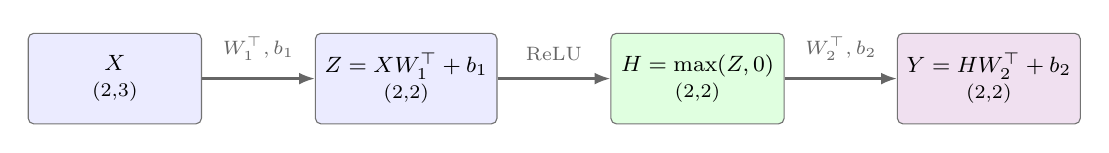
\begin{tikzpicture}[font=\footnotesize,
    blk/.style={draw=black!55, rounded corners=2pt, minimum width=2.2cm,
                minimum height=1.15cm, fill=blue!8, align=center},
    arr2/.style={-{Latex[length=2mm]}, thick, black!60}]
  \node[blk] (fx) at (0,0)    {$X$\\ \scriptsize (2,3)};
  \node[blk] (fz) at (3.7,0)  {$Z = X W_1^{\top} + b_1$\\ \scriptsize (2,2)};
  \node[blk, fill=green!12] (fh) at (7.4,0) {$H = \max(Z, 0)$\\ \scriptsize (2,2)};
  \node[blk, fill=violet!12] (fy) at (11.1,0) {$Y = H W_2^{\top} + b_2$\\ \scriptsize (2,2)};
  \draw[arr2] (fx) -- (fz) node[midway, above=1mm, font=\scriptsize] {$W_1^{\top}, b_1$};
  \draw[arr2] (fz) -- (fh) node[midway, above=1mm, font=\scriptsize] {ReLU};
  \draw[arr2] (fh) -- (fy) node[midway, above=1mm, font=\scriptsize] {$W_2^{\top}, b_2$};
\end{tikzpicture}
\caption{NP-M4 前向计算的 shape 链路：线性 $\rightarrow$ ReLU $\rightarrow$ 线性；每步 shape 固定，bias 沿行广播}
\label{fig:forward}
\end{figure}

\subsection{数值安全：clip、nan 与 ValueError}

$\arccos$ 的定义域是 $[-1,1]$，而浮点运算常常给出 \code{1.0000000000000002} 这样的值，直接送进 \code{np.arccos} 会得到 \code{nan} 并打印警告。因此所有求夹角的地方都在求反余弦前用 \code{np.clip} 截断，再把“零向量无方向”这一数学事实翻译成两种不同的程序语义（表~\ref{tab:edge}）：查询向量为零时是调用者的错误，抛 \code{ValueError}；被比较的行中某行为零时只是该行无定义，返回 \code{nan} 并保持数组形状不变。

\begin{lstlisting}[caption={NP-M1：批量夹角中的 clip 与 nan 处理（原样片段）}, label={lst:m1}]
dianji = juzhen @ chaxun                          # 一次矩阵乘得到所有点乘
changdu_juzhen = np.linalg.norm(juzhen, axis=1)   # 按行求长度
fenmu = changdu_juzhen * changdu_chaxun
fenmu_safe = np.where(fenmu == 0, 1.0, fenmu)    # 零行分母先换 1，避免除零
yuxian = np.clip(dianji / fenmu_safe, -1.0, 1.0)
jiaodu = np.degrees(np.arccos(yuxian))
jiaodu = np.where(changdu_juzhen == 0, np.nan, jiaodu)   # 零行覆盖为 nan
\end{lstlisting}

\subsection{不修改输入}

\code{unit\_vector} 采用 \code{v / norm}（生成新数组）而不是 \code{v /= norm}（原地修改）；E1 的“负数置 0”先 \code{A.copy()} 再掩码赋值，避免 \code{B = A} 这种别名写法连带改掉原数组；M4 只读参数、不写参数。这三处都在运行结果中做了显式核对。

\section{Results}

全部 12 道题在 Python 3.13.14 + NumPy 2.5.5 下运行通过，关键数值如表~\ref{tab:results}，与报告中解析计算的结果一致。

\begin{table}[H]
\centering
\small
\setlength{\tabcolsep}{4pt}
\caption{12 道题的关键输出（表中保留 6 位小数）}
\label{tab:results}
\begin{tabular}{@{}l p{10.2cm} p{2.0cm}@{}}
\toprule
\textbf{题目} & \textbf{输出数值（保留 6 位小数）} & \textbf{shape} \\
\midrule
NP-E1 & \code{ndim=2, shape=(3,4), size=12}；\code{A[1]=[0.80,0.30,-0.70,0.60]} & \code{(4,)} \\
      & \code{A[:, -2:]=[[1.10,0.40],[-0.70,0.60],[0.10,-0.20]]} & \code{(3,2)} \\
      & \code{B}（负数置 0）第 1 行 \code{[0.80,0.30,0.00,0.60]}，\code{A} 保持原值 & \code{(3,4)} \\
NP-E2 & \code{a*b=[-0.16,-0.54,0.28]}；\code{a@b=-0.42} & \code{(3,)} / \code{()} \\
      & \code{||a||=1.220656}，\code{||b||=1.004988}（与 \code{np.linalg.norm} 完全一致） & \code{()} \\
NP-E3 & \code{angle\_deg(a,b)=45.000000}；零向量输入抛 \code{ValueError} & \code{()} \\
NP-E4 & \code{p-q=[-1.30,1.60,0.90]}；欧氏 \code{2.249444}；曼哈顿 \code{3.800000} & \code{(3,)} \\
NP-E5 & \code{u=[-0.801784,0.267261,0.534522]}，\code{||u||=1}，\code{allclose} 通过 & \code{(3,)} \\
NP-E6 & \code{sum(axis=0)=[1.00,-0.10,0.80]}；\code{mean(axis=1)=[0.266667,0.300000]} & \code{(3,)} / \code{(2,)} \\
      & 全局最大值 \code{1.10}，位置 \code{(0,2)}（第 1 行第 3 列） & \code{()} \\
NP-E7 & \code{Y=[[1.10,-0.10,-0.40],[-0.70,0.45,0.10]]} & \code{(2,3)} \\
NP-E8 & \code{batch} 共 24 个元素；蓝通道（C=2）取 \code{batch[:,2]}，两个 $2\times2$ 平面 & \code{(2,3,2,2)} \\
      & 转 \code{(B,H,W,C)} 顺序后 & \code{(2,2,2,3)} \\
NP-M1 & \code{[0.000000, 180.000000, 90.000000, nan]}（同向 / 反向 / 正交 / 零向量） & \code{(4,)} \\
NP-M2 & \code{idx=[0,1,2]}，\code{sim=[1.000000,1.000000,0.000000]} & \code{(3,)} \\
      & Top-3 ID：\code{img\_a}、\code{img\_b}、\code{img\_c}，零向量行 \code{img\_zero} 被排除 & \\
NP-M3 & \code{D=[[0.608276,0.824621],} & \code{(3,2)} \\
      & \code{~~[0.707107,1.486607],} & \\
      & \code{~~[0.781025,0.905539]]} & \\
      & 最近邻索引 \code{[0,0,0]}，与双重循环版本 \code{allclose} 一致 & \code{(3,)} \\
NP-M4 & \code{Z=[[-0.91,0.66],[-0.93,0.27]]} & \code{(2,2)} \\
      & \code{H=[[0.00,0.66],[0.00,0.27]]}（两个负值被 ReLU 置 0） & \code{(2,2)} \\
      & \code{Y=[[-0.2960,0.1432],[-0.0620,-0.0596]]} & \code{(2,2)} \\
\bottomrule
\end{tabular}
\end{table}

\textbf{边界输入的实测行为}如表~\ref{tab:edge} 所示，全部异常都由代码主动抛出并给出中文提示，而不是让 NumPy 抛底层警告。

\begin{table}[H]
\centering
\small
\setlength{\tabcolsep}{4pt}
\caption{边界输入的处理方式（实测）}
\label{tab:edge}
\begin{tabular}{@{}l l p{6.4cm}@{}}
\toprule
\textbf{位置} & \textbf{边界输入} & \textbf{实测行为} \\
\midrule
\code{angle\_deg} & \code{a=[0,0]} & \code{ValueError}：零向量没有方向，夹角无定义 \\
\code{unit\_vector} & \code{[0,0,0]} & \code{ValueError}：零向量无法归一化 \\
\code{angles\_to} & \code{query=[0,0,0]} & \code{ValueError}：query 是零向量，夹角无定义 \\
\code{angles\_to} & $X$ 第 3 行为零向量 & 第 3 个位置返回 \code{nan}，其余 3 个角度正常 \\
\code{top\_k\_cosine} & \code{k=0}，或 \code{k=9} 超过有效行数 4 & \code{ValueError}：k 必须在 1..4 之间 \\
\code{top\_k\_cosine} & 分数并列（\code{img\_a}、\code{img\_b} 均为 1.0） & 稳定排序，保持原行序（\code{a} 在 \code{b} 前） \\
\bottomrule
\end{tabular}
\end{table}

\section{Discussion}

\textbf{1. 广播是最容易出错、也最值得理解的一步。} 写 E7 时如果只记住“能乘”，很容易在 M4 里把 \code{X @ W1.T} 写成 \code{X @ W1} 而得到 shape 错误；M3 若不插轴直接 \code{A - B}，会因为 \code{(3,2)} 与 \code{(2,2)} 恰好可广播而得到“逐元素相减”的错误结果——它不报错，但语义完全不对。所以本作业坚持每步先写 shape 再写代码。

\textbf{2. axis 是“被压缩掉的轴”。} \code{sum(axis=0)} 之后 shape 从 \code{(2,3)} 变成 \code{(3,)}，消失的正是行维，因此它对应“每一列一个汇总值”；记住这一点，E6 的“结果对应哪些输入位置”就不再需要背。

\textbf{3. 浮点误差必须先处理再求反三角函数。} 实测 \code{angle\_deg} 返回 \code{45.00000000000001}，而如果不做 \code{clip}，\code{img\_a} 那种“与 query 完全同向”的行会算出 \code{cos=1.0000000000000002}，\code{arccos} 直接给 \code{nan}。\code{clip} 只用了两个边界值，却把一整类隐性 \code{nan} 消除了。

\textbf{4. \code{nan} 会静默传播，比较时要用 \code{np.isnan}。} M1 中先用 \code{np.where} 把零行分母替换为 1 避免除零、再用 \code{np.where} 把零行结果覆盖为 \code{nan} 的写法，保证输出顺序与 $X$ 的行顺序严格对应；若改用 \code{np.nan\_to\_num} 或布尔索引压缩数组，形状会悄悄从 \code{(4,)} 变成 \code{(3,)}。

\textbf{5. 向量化换来的是代码简洁与常数因子，不是算法复杂度。} M3 的广播仍是 $O(MND)$ 次运算，只是把循环交给 C 层；代价是 \code{(M,N,D)} 的中间数组，$M=N=10^4$ 时会占用数 GB 内存，工程上需要分块。这是“一条表达式”的边界，也是下一步可以改进的地方（用 \code{scipy.spatial.distance.cdist} 或分块累加）。

\textbf{6. 可改进之处}：目前各题直接用 \code{print} 输出结果，缺少自动断言；若时间允许，可为每个函数补 \code{assert np.allclose(...)} 形式的轻量单元测试，把“报告里的数字”变成“能自动回归的测试”。

\section{Links and References}

\begin{itemize}
    \item \textbf{代码仓库}：\code{https://github.com/jiapanjbd/project1\_numpy}（README 含一键复现步骤与结果摘要）；
    \item \textbf{提交版本}：\code{9944a66}（本报告所用代码版本对应的 7 位提交哈希，见仓库提交记录）；
    \item \textbf{运行环境}：Windows 11，Python 3.13.14，NumPy 2.5.5，无其他第三方依赖；主要参数即题目给定数组，全部内置在 \code{numpy\_homework.py} 中；
    \item \textbf{参考与工具声明}：题目数据与指定函数名来自课程讲义，报告版式基于 SZU 实验报告模版；12 道题目的实现、调试与结果核对由本人完成，代码合并、README 与报告框架借助 AI 辅助生成。
\end{itemize}

\newpage

% ============================================================
% 批阅与成绩评定页
% ============================================================
\begin{tikzpicture}[remember picture, overlay]
  \draw[thick]
    ($(current page.north west)+(2cm,-3cm)$)
    rectangle
    ($(current page.south east)+(-2cm,3.5cm)$);
\end{tikzpicture}

\vspace{1cm}

\noindent \textbf{指导教师批阅意见：}
\vspace{6cm}
\hfill

\vspace{1cm}

\noindent \textbf{成绩评定：}
\vspace{2cm}
\hfill

\vspace{1cm}

\noindent
\hfill
\textbf{指导教师签字：}\quad\quad\quad\quad\quad\\[0.5cm]

\hfill
\textbf{年}\quad\quad
\textbf{月}\quad\quad
\textbf{日}\quad

\vspace{1cm}

\noindent \textbf{备注：}

\begin{tikzpicture}[remember picture, overlay]
  \node[
    anchor=north west,
    inner sep=0pt,
    text width=\dimexpr\paperwidth-4cm\relax
  ] at ($(current page.south west)+(2cm,3.1cm)$) {
    \begin{minipage}{\dimexpr\paperwidth-4cm\relax}
      \small
      \noindent
      \textbf{注：}\;1、报告内的项目或内容设置，可根据实际情况加以调整和补充。\\[0.2cm]
      \phantom{\textbf{注：}\;}2、教师批改学生实验报告时间应在学生提交实验报告时间后 10 日内。
    \end{minipage}
  };
\end{tikzpicture}

\end{document}
